\subsection{随机变量}
\paragraph{}
有些试验的样本空间不是数字类型,因此可通过将样本空间映射到实数上,研究样本的概率分布情况。比如:硬币的$\{H,T\} \to \{0, 1\}$
\paragraph{}
\textbf{定义\;}设随机试验的样本空间为$S=\{e\}$。$X = X(e)$是定义在样本空间$S$上的实值单值函数,称$X=X(e)$为随机变量。

\paragraph{}
实值单值函数,比如:$y=f(x)$,实值即$x$的定义域是实数集合$R$;单值函数即$x$对应的$y$是唯一的。

\subsection{离散型随机变量及其\textbf{分布律}}
\subsubsection{离散型随机变量}
\paragraph{}
有些随机变量,它全部可能取到的值是有限个或可列无限多个,这种随机变量称为\textbf{离散型随机变量}。

\paragraph{}
设离散型随机变量$X$所有可能取的值为$x_k(k=1,2,\cdots)$,$X$取各个可能值的概率,即事件$\{X = x_k\}$的概率,为:
\begin{equation}
  \label{离散型随机变量的分布律}
  P\{X = x_k\} = p_k, k = 1, 2, \cdots.
\end{equation}
由概率的定义,$p_k$满足如下两个条件:

\label{离散型随机变量的条件}
\begin{enumerate}
  \item $p_k \geq 0, k = 1, 2, \cdots$
  \item $\displaystyle \sum_{k=1}^\infty p_k = 1$
\end{enumerate}
我们称 \eqref{离散型随机变量的分布律} 式为离散型随机变量$X$的\textbf{分布律},分布律也可以用表格的形式表示:

\begin{figure}[H]
\centering
  \begin{tabular}{c|ccccc}
    $X$ & $x_1$ & $x_2$ & $\cdots$ & $x_n$ & $\cdots$ \\
    \hline
    \\ [-1em]
    $p_k$ & $p_1$ & $p_2$ & $\cdots$ & $p_n$ & $\cdots$ \\
  \end{tabular}
\end{figure}

\subsubsection{(0-1)分布}
\paragraph{}
设随机变量$X$只可能取$0$与$1$两个值,它的分布律是:

\begin{equation}
  P\{X=k\}=p^k(1-p)^{1-k},k=0,1(0<p<1)
\end{equation}

则称$X$服从以$p$为参数的(0-1)分布或两点分布,以下以表格形式表示:

\begin{figure}[H]
\centering
  \begin{tabular}{c|cc}
    $X$ & $0$ & $1$ \\
    \hline
    \\ [-1em]
    $p_k$ & $1-p$ & $p$ \\
  \end{tabular}
\end{figure}

\subsubsection{伯努利试验、二项分布}
\paragraph{}
设试验$E$只有两个可能结果:$A$及$\overline{A}$,则称$E$为\textbf{伯努利(Bernoulli)试验}。设$P(A) = p(0<p<1)$,此时$P(\overline{A})=1-p$。将$E$独立重复地进行$n$次,则称这一串重复地独立试验为\textbf{$n$重伯努利试验}。

\paragraph{}
“重复”是指在每次试验中$P(A)=p$保持不变;“独立”是指各次试验的结果互不影响。若以$C_i$记第$i$次试验的结果,$C_i$为$A$或$\overline{A}, i = 1,2,\cdots,n$,“独立”是指:
\begin{equation}
  P(C_1C_2\cdots C_n) = P(C_1)P(C_2)\cdots P(C_n).
\end{equation}

\paragraph{}
以$X$表示$n$重伯努利试验中事件$A$发生的次数,$X$是一个随机变量。$X$所有可能取的值为$0,1,2,\cdots,n$。由于各次试验是相互独立的,因此事件$A$在指定的$k(0 \leq k \leq n)$次试验中发生,在其它$n-k$次试验中$A$不发生,前$k$次试验中$A$发生而后$n-k$次试验中$A$不发生的概率为:

\begin{equation}
  % \bigcdot 额外配置的命令
  \underbrace{p \bigcdot p \bigcdot \cdots \bigcdot p}_{k \text{个}} \bigcdot \underbrace{(1-p) \bigcdot (1-p) \bigcdot \cdots \bigcdot (1-p)}_{n-k \text{个}} = p^k(1-p)^{n-k}.
\end{equation}

这种指定的方式共有${{n}\choose{k}}$种,它们是两两互不相容的,故在$n$次试验中$A$发生$k$次的概率为${{n}\choose{k}}p^k(1-p)^{n-k}$,记$q = 1 - p$,即有:

\begin{equation}
  P\{X=k\} = {{n}\choose{k}}p^kq^{n-k}, k=0,1,2,\cdots,n.
\end{equation}
显然
\begin{gather}
  P\{X=k\} \geq 0, k = 0,1,2,\cdots,n; \\
  \sum_{k=0}^nP\{X=k\} = \sum_{k=0}^n {{n}\choose{k}}p^kq^{n-k}=(p+q)^n = 1.
\end{gather}
即$P\{X=k\}$满足 \hyperref[离散型随机变量的条件]{\color{blue} \ref*{离散型随机变量的条件}} 的两个条件,注意到${{n}\choose{k}}p^kq^{n-k}$刚好是二项式$(p+q)^n$的展开式中出现$p^k$的那一项,我们称随机变量$X$服从参数为$n,p$的\textbf{二项分布},并记为$X \thicksim b(n,p)$。

\paragraph{}
特别地,当$n=1$时,二项分布变成(0-1)分布。

\subsubsection{泊松分布}
\paragraph{}
设随机变量$X$所有可能取的值为$0,1,2,\cdots$,而取各个值的概率为

\begin{equation}
  P\{X=k\} = \frac{\lambda^ke^{-\lambda}}{k!}, k = 0,1,2,\cdots,
\end{equation}

其中$\lambda > 0$是常数。则称$X$服从参数为$\lambda$的\textbf{泊松分布},记为$X\thicksim \pi(\lambda)$

\paragraph{}
\textbf{泊松定理\;}设$\lambda>0$是一个常数,$n$是任意正整数,设$np_n=\lambda$,则对于任一固定的非负整数$k$,有

\begin{equation}
  \lim_{n \to \infty} {n \choose k}p_n^k(1-p)^{n-k}=\frac{\lambda^ke^{-\lambda}}{k!}.
\end{equation}

\subsection{随机变量的\textbf{分布函数}}
\paragraph{}
非离散型随机变量$X$,其取值不能一一列举出来,因此不能用分布律来描述它。实际中,研究误差落在某个区间,而不是具体某个样本,由于

\begin{equation}
  P\{x_1<X\leq x_2\} = P\{X\leq x_2\} - P\{X \leq x_1\},
\end{equation}

我们只需知道$P\{X\leq x_2\}$和$P\{X \leq x_1\}$,即可知道落在区间$(x_1,x_2]$的概率了。

\paragraph{}
\textbf{定义\;}设$X$是一个随机变量,$x$是任意实数,函数

\begin{equation}
  F(x) = P\{X \leq x\}, -\infty < x < \infty
\end{equation}

称为$X$的\textbf{分布函数}。

\paragraph{}
对于任意实数$x_1, x_2 (x_1 < x_2)$,有

\begin{align}
  \begin{split}
    P\{x_1 < X \leq x_2\} =&\; P\{X \leq x_2\} - P\{X \leq x_1\} \\
    =&\; F(x_2) - F(x_1)
  \end{split}
\end{align}

\paragraph{}
分布函数$F(x)$具有以下的基本性质:

\begin{enumerate}
  \item $F(x)$是一个不减函数,由$F(x_2) - F(x_1) = P\{x_1 < X \leq x_2\} \geq 0$可证明,也称为累计分布函数
  \item $0 \leq F(x) \leq 1$,且
  \begin{align}
    \begin{split}
      F(-\infty) =&\; \lim_{x \to -\infty}F(x) = 0, \\
      F(\infty) =&\; \lim_{x \to \infty}F(x) = 1. \\
    \end{split}
  \end{align}
  \item $F(x+0) = F(x)$,即$F(x)$是右连续的。
\end{enumerate}

\subsection{连续型随机变量及其概率密度}
\paragraph{}
如果对于随机变量$X$的分布函数$F(x)$,存在非负函数$f(x)$,使对于任意实数$x$有

\begin{equation}
  \label{连续型随机变量的分布函数}
  F(x) = \int_{-\infty}^{x}f(t)dt,
\end{equation}
则称$X$为\textbf{连续型随机变量},其中函数$f(x)$称为$X$的\textbf{概率密度函数},简称\textbf{概率密度}。

\paragraph{}
概率密度$f(x)$具有以下性质:
\begin{enumerate}
  \item $f(x) \geq 0$
  \item $\int_{-\infty}^{\infty}f(x)dx=1$
  \item 对于任意实数$x_1, x_2(x_1 \leq x_2),$
  \begin{equation}
    P\{x_1 < X \leq x_2\} = F(x_2) - F(x_1) = \int_{x_1}^{x_2}f(x)dx
  \end{equation}
  \item 若$f(x)$在点$x$处连续,则有$F'(x) = f(x)$
\end{enumerate}

\begin{figure}[h]
\centering
  %------- 第1行 -------
  \begin{subfigure}[t]{0.48\linewidth}
    \centering
      % 1.05*e^(-(x+1)^2) + 0.8*e^(-(x-1)^2) + 0.1
\begin{tikzpicture}[scale = 0.9]
  \begin{axis}[clip=false,xmin=-4.5,xmax=4.5,ymin=-0.15,ymax=1.6,ticks=none,axis lines=middle,smooth,xlabel={$x$}, ylabel={$f(x)$}]
    \addplot[draw=blue,domain=-4.5:4,samples=200] {1.05*e^(-(x+1)^2) + 0.8*e^(-(x-1)^2) + 0.1};
    \addplot+[draw=none,mark=none,domain=-4.5:4,samples=100,%
              pattern=north east lines]%
              {1.05*e^(-(x+1)^2) + 0.8*e^(-(x-1)^2) + 0.1}
              \closedcycle;
    \node[fill=white] at (-1,0.5) {$1$};
    \node[below left] at (0,0) {$O$};
  \end{axis}
\end{tikzpicture}

  \end{subfigure}
  \begin{subfigure}[t]{0.48\linewidth}
    \centering
      % 2 * e^(-(x+1)^2) + 1.5* e^(-(x-1)^2) + 0.1
\begin{tikzpicture}[scale = 0.9]
  \begin{axis}[clip=false,xmin=-4.5,xmax=4.5,ymin=-0.15,ymax=1.6,ticks=none,axis lines=middle,smooth,xlabel={$x$}, ylabel={$f(x)$}]
    \addplot[draw=blue,domain=-4.5:4,samples=200] {1.05*e^(-(x+1)^2) + 0.8*e^(-(x-1)^2) + 0.1};
    \addplot+[draw=blue,mark=none,domain=0.6:1.2,samples=100,%
              pattern=north east lines]%
              {1.05*e^(-(x+1)^2) + 0.8*e^(-(x-1)^2) + 0.1}
              \closedcycle;
    \node at (-1,0.5) {$1$};
    \node[below left] at (0,0) {$O$};
    \node[below] at (0.6,0) {$x_1$};
    \node[below] at (1.2,0) {$x_2$};
  \end{axis}
\end{tikzpicture}

  \end{subfigure}
  \caption{概率密度性质}
  \label{概率密度性质}
\end{figure}

\paragraph{}
由\textbf{性质4}在$f(x)$的连续点$x$处有

\begin{align}
  \label{f(x)连续性质}
  \begin{split}
    f(x) =&\; \lim_{\Delta x \to 0^+}\frac{F(x+\Delta x) - F(x)}{\Delta x} \\
    =&\; \lim_{\Delta x \to 0^+}\frac{P\{x < X \leq x + \Delta x\}}{\Delta x}.
  \end{split}
\end{align}

\paragraph{}
由 \eqref{f(x)连续性质} 式知道,若不计高阶无穷小,有

\begin{equation}
  P\{x < X \leq x + \Delta x\} \approx f(x)\Delta x.
\end{equation}

这表示$X$落在小区间$(x, x+\Delta x]$上的概率近视地等于$f(x)\Delta x$.

\paragraph{}
对于连续型随机变量$X$来说,它取任一指定实数值$a$的概率均为$0$,即$P\{X=a\}=0$,因此可以不必区分该区间是开区间或闭区间:

\begin{equation}
  P\{a < X \leq b\} = P\{a \leq X \leq b\} = P\{a < X < b\}.
\end{equation}

\paragraph{}
下面介绍三种重要的连续型随机变量。

\subsubsection{均匀分布}
\paragraph{}
若连续型随机变量$X$具有概率密度

\begin{equation}
  f(x) = \left\{ \begin{array}{ll}
    \frac{1}{b-a}, & a<x<b, \\
    0, & \textbf{\small 其它},
  \end{array}\right.
\end{equation}

则称$X$在区间$(a,b)$上服从\textbf{均匀分布}。记为$X \sim U(a,b)$

\paragraph{}
对于任一长度$l$的子区间$(c, c+l), a \leq c < c+l \leq b$,有

\begin{equation}
  P\{c < X \leq c+l\} = \int_c^{c+l}f(x)dx = \int_c^{c+l}\frac{1}{b-a}dx=\frac{l}{b-a}.
\end{equation}

\paragraph{}
由 \eqref{连续型随机变量的分布函数} 式得$X$的分布函数为:

\begin{equation}
  F(x) = \left\{ \begin{array}{ll}
    0, & x < a, \\
    \frac{x-a}{b-a}, & a \leq x < b, \\
    1, & x \geq b.
  \end{array} \right.
\end{equation}

\paragraph{}
$f(x)$及$F(x)$的图形分别为:

\begin{figure}[h]
\centering
  %------- 第1行 -------
  \begin{subfigure}[t]{0.48\linewidth}
    \centering
      % 均匀分布
\begin{tikzpicture}
  \begin{axis}[clip=false,xmin=0,xmax=3,ymin=0,ymax=1.5,ticks=none,axis lines=middle,y=2cm,x=1.5cm,smooth,xlabel={$x$}, ylabel={$f(x)$}]

    \addplot[draw=blue,domain=1:2,samples=2,thick] {0.5};
    \addplot[draw=blue,domain=0:1,samples=2,thick] {0};
    \addplot[draw=blue,domain=2:3,samples=2,thick] {0};

    \draw[dashed] (1,0) -- (1,0.5);
    \draw[dashed] (2,0) -- (2,0.5);

    % y label
    \draw (0,0.5) -- (0.05,0.5);
    \node[left] at (0,0.5) {$\frac{1}{b-a}$};

    \node[below] at (1,0) {$a$};
    \node[below] at (2,0) {$b$};
    \node[below left] at (0,0) {$O$};
  \end{axis}
\end{tikzpicture}

  \end{subfigure}
  \begin{subfigure}[t]{0.48\linewidth}
    \centering
      % 均匀分布
\begin{tikzpicture}
  \begin{axis}[clip=false,xmin=0,xmax=3,ymin=0,ymax=1.5,ticks=none,axis lines=middle,y=2cm,x=1.5cm,smooth,xlabel={$x$}, ylabel={$F(x)$}]

    \addplot[draw=blue,domain=1:2,samples=2,thick] {x-1};
    \addplot[draw=blue,domain=0:1,samples=2,thick] {0};
    \addplot[draw=blue,domain=2:3,samples=2,thick] {1};

    % y label
    \draw (0,1) -- (0.05,1);
    \node[left] at (0,1) {$1$};

    \node[below] at (1,0) {$a$};
    \node[below] at (2,0) {$b$};
    \node[below left] at (0,0) {$O$};
  \end{axis}
\end{tikzpicture}

  \end{subfigure}
  \caption{均匀分布的概率密度及其分布函数}
  \label{均匀分布的概率密度及其分布函数}
\end{figure}

\subsubsection{指数分布}
\paragraph{}
若连续型随机变量$X$的概率密度为:
\begin{equation}
  \label{指数分布的概率密度公式}
  f(x) = \left\{ \begin{array}{ll}
    \frac{1}{\theta}e^{-x/\theta}, & x > 0 \\ 0, & \text{其它,}
  \end{array} \right.
\end{equation}

其中$\theta > 0$为常数,则称$X$服从参数为$\theta$的\textbf{指数分布}。

\begin{figure}[H]
  \centering
    % 指数分布概率密度函数
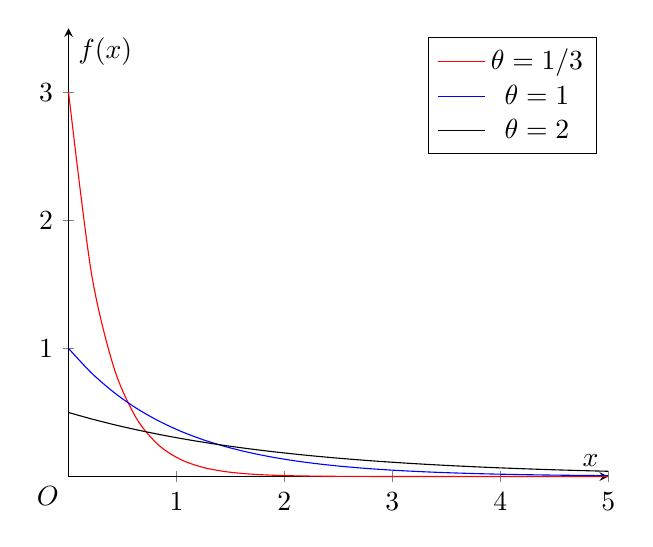
\begin{tikzpicture}
  \begin{axis}[clip=false,xmin=0, xmax=5,ymin=0,ymax=3.5, axis lines = middle,
    smooth, xlabel={$x$}, ylabel={$f(x)$}]
    \addplot[draw=red,domain=0:5] {3*e^(-3*x)};
    \addplot[draw=blue,domain=0:5] {e^(-x)};
    \addplot[draw=black,domain=0:5] {0.5*e^(-x*0.5)};
    \node[below left] at (0,0) {$O$};

    \addlegendentry{$\theta=1/3$}
    \addlegendentry{$\theta=1$}
    \addlegendentry{$\theta=2$}
  \end{axis}
\end{tikzpicture}

    \caption{指数分布的概率密度函数}
    \label{指数分布的概率密度函数}
\end{figure}

\paragraph{}
由 \eqref{指数分布的概率密度公式} 式得到随机变量$X$的分布函数为:

\begin{equation}
  F(x) = \left\{ \begin{array}{ll}
    1 - e^{-x/\theta}, & x > 0 \\ 0, & \text{其它}
  \end{array} \right.
\end{equation}

\paragraph{}
\textbf{无记忆性}性质:对于任意$s,t>0$,有

\begin{equation}
  P\{X > s + t \;|\; X > s\} = P\{X > t\}.
\end{equation}

\subsubsection{正态分布}
\paragraph{}
若连续型随机变量 X 的概率密度为

\begin{equation}
  \label{正态分布公式}
  f(x) = \frac{1}{\sqrt{2\pi}\sigma}e^{-\frac{(x-\mu)^2}{2\sigma^2}}, -\infty < x < \infty,
\end{equation}

其中$\mu, \sigma(\sigma > 0)$为常数,则称$X$服从参数为$\mu, \sigma$的\textbf{正态分布}或\textbf{高斯}分布,记为$X\sim N(\mu, \sigma^2)$.

\paragraph{}
\textbf{性质:}
\begin{enumerate}
  \item 曲线关于$x=\mu$对称,对于任意$h > 0$有
  \begin{equation}
    P\{\mu-h < X \leq \mu\} = P\{\mu < X \leq \mu+h\}.
  \end{equation}
  \item 当$x=\mu$时取到最大值
  \begin{equation}
    f(\mu) = \frac{1}{\sqrt{2\pi}\sigma}.
  \end{equation}
\end{enumerate}

\paragraph{}
\begin{figure}[H]
\centering
  %------- 第1行 -------
  \begin{subfigure}[t]{0.48\linewidth}
    \centering
      % 正态分布概率密度函数,\mu参数的变化情况
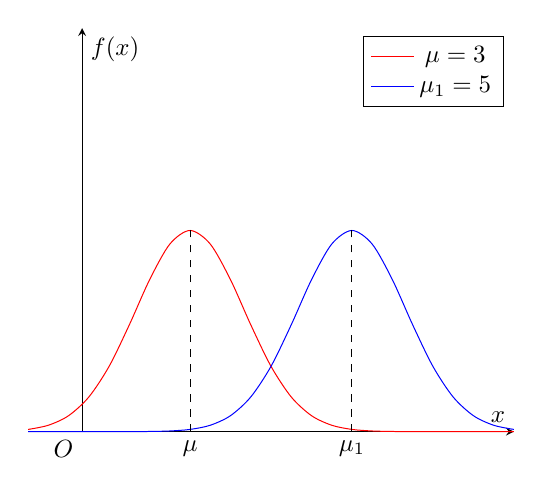
\begin{tikzpicture}[scale = 0.9]
  \begin{axis}[clip=false,xmin=-1, xmax=8,ymin=0,ymax=0.8, axis lines = middle,
    smooth, xlabel={$x$}, ylabel={$f(x)$},ticks=none]
    % mu = 2, sigma = 1
    \addplot[draw=red,domain=-1:8] {0.3989 * e^(-((x-2)^2)/2)};
    % mu = 5, sigma = 1
    \addplot[draw=blue,domain=-1:8] {0.3989 * e^(-((x-5)^2)/2)};

    % x = 2,中心
    \draw[dashed] (2,0) -- (2,0.3989);
    \node[below] at (2,0) {$\mu$};
    % x = 5,中心
    \draw[dashed] (5,0) -- (5,0.3989);
    \node[below] at (5,0) {$\mu_1$};

    % 原点标签
    \node[below left] at (0,0) {$O$};

    % 图示
    \addlegendentry{$\mu=3$}
    \addlegendentry{$\mu_1=5$}
  \end{axis}
\end{tikzpicture}

  \end{subfigure}
  \begin{subfigure}[t]{0.48\linewidth}
    \centering
      % 正态分布概率密度函数,\sigma参数的变化情况
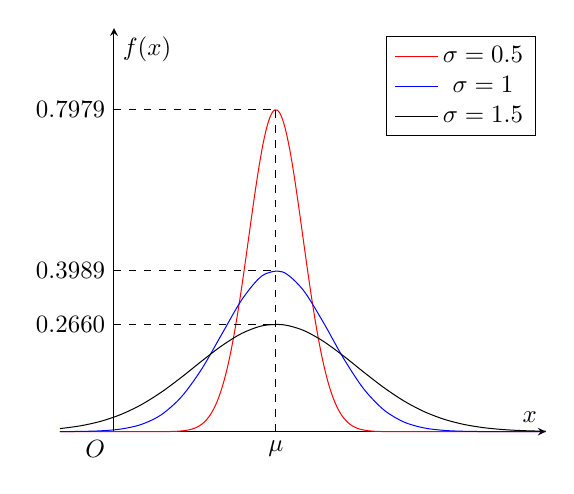
\begin{tikzpicture}[scale = 0.9]
  \begin{axis}[clip=false,xmin=-1, xmax=8,ymin=0,ymax=1, axis lines = middle,
    smooth, xlabel={$x$}, ylabel={$f(x)$},ticks=none]
    % mu = 3, sigma = 0.5
    \addplot[draw=red,domain=-1:8,samples=200] {0.7979 * e^(-((x-3)^2)/0.5)};
    % mu = 3, sigma = 1
    \addplot[draw=blue,domain=-1:8] {0.3989 * e^(-((x-3)^2)/2)};
    % mu = 3, sigma = 1.5
    \addplot[draw=black,domain=-1:8] {0.2660 * e^(-((x-3)^2)/4.5)};

    % y = 0.7979, [0,3],最高点
    \draw[dashed] (0,0.7979) -- (3,0.7979);
    \node[left] at (0,0.7979) {$0.7979$};
    % y = 0.3989, [0,3],最高点
    \draw[dashed] (0,0.3989) -- (3,0.3989);
    \node[left] at (0,0.3989) {$0.3989$};
    % y = 0.2660, [0,3],最高点
    \draw[dashed] (0,0.2660) -- (3,0.2660);
    \node[left] at (0,0.2660) {$0.2660$};

    \draw[dashed] (3,0) -- (3,0.7978);
    \node[below] at (3,0) {$\mu$};

    % 原点标签
    \node[below left] at (0,0) {$O$};

    % 图示
    \addlegendentry{$\sigma=0.5$}
    \addlegendentry{$\sigma=1$}
    \addlegendentry{$\sigma=1.5$}
  \end{axis}
\end{tikzpicture}

  \end{subfigure}
  \caption{正态分布的概率密度函数}
  \label{正态分布的概率密度函数}
\end{figure}

\paragraph{}
由 \eqref{正态分布公式} 式得$X$的分布函数为
\begin{equation}
  F(x) = \frac{1}{\sqrt{2\pi}\sigma}\int_{-\infty}^x e^{\frac{(t-\mu)^2}{2\sigma^2}}dt,
\end{equation}

特别地,当$\mu=0, \sigma=1$时,称随机变量$X$服从\textbf{标准正态分布},其概率密度和分布函数分别用$\varphi(x), \Phi(x)$表示,而且易知:
\begin{equation}
  \Phi(-x) = 1 - \Phi(x)
\end{equation}

\begin{figure}[H]
\centering
  %------- 第1行 -------
  \begin{subfigure}[t]{0.48\linewidth}
    \centering
      % 正态分布的分布函数
\begin{tikzpicture}[scale = 0.9]
  \begin{axis}[clip=false,xmin=-4, xmax=6,ymin=0,ymax=1.5, axis lines = middle,
    smooth, xlabel={$x$}, ylabel={$F(x)$},ticks=none]
    % 用近似公式画图,F(x) = e^(a(x-u)) / (1 + e^(a(x-u))), a = 4 / sigma * sqrt(2*pi)
    % sigma = 1, mu = 0.7
    \addplot[draw=red,domain=-4:6, samples=200] {e^(1.5957 * (x-0.7)) / (1 + e^(1.5957 * (x-0.7)))};

    % 原点标签
    \node[below left] at (0,0) {$O$};

    % y = 1 刻度
    \draw[dashed] (0,1) -- (0.2,1);
    \node[left] at (0,1) {$1$};

    % (0.7, 0.5) 坐标的辅助线
    \draw[dashed] (0,0.5) -- (0.7,0.5);
    \draw[dashed] (0.7,0) -- (0.7,0.5);
    \node[left] at (0,0.5) {$0.5$};
    \node[below] at (0.7,0) {$\mu$};
  \end{axis}
\end{tikzpicture}

      \caption{正态分布的分布函数}
  \end{subfigure}
  \begin{subfigure}[t]{0.48\linewidth}
    \centering
      % 标准正态分布的概率密度函数
\begin{tikzpicture}[scale = 0.9]
  \begin{axis}[clip=false,xmin=-4, xmax=4,ymin=0,ymax=0.6, axis lines = middle,
    smooth, xlabel={$x$}, ylabel={$f(x)$},ticks=none]
    % mu = 0, sigma = 1
    \addplot[draw=red,domain=-4:4] {0.3989 * e^(-x^2/2)};

    % x=-2, x=2
    \draw[dashed] (-2,0) -- (-2,0.053);
    \draw[dashed] (2,0) -- (2,0.053);
    \node[below] at (-2,0) {$-x$};
    \node[below] at (2,0) {$x$};

    % 原点标签
    \node[below left] at (0,0) {$O$};
  \end{axis}
\end{tikzpicture}

      \caption{标准正态分布的概率密度函数}
  \end{subfigure}
  \caption{分布函数及标准正态分布的密度函数}
  \label{分布函数及标准正态分布的密度函数}
\end{figure}

\subsection{随机变量的函数的分布}
\paragraph{}
在一些试验中,所关心的随机变量往往不能直接测量得到,而它却是某个能直接测量的随机变量的函数。\textbf{比如:}我们能测量圆轴截面的直径$d$,而关心的却是截面面积$A=\frac{1}{4}\pi d^2$。

\paragraph{}
\textbf{定理\quad}设随机变量$X$具有概率密度$f_X(x), -\infty < x < \infty$,又设函数$g(x)$处处可导且恒有$g'(x)>0$(或恒有$g'(x)<0$),则$Y=g(X)$是连续型随机变量,其概率密度为

\begin{equation}
  f_Y(y) = \left\{ \begin{array}{ll}
    f_X[h(y)]|h'(y)|, & \alpha < y < \beta, \\ 0, & \text{其它,}
  \end{array}\right.
\end{equation}

其中$\alpha=min\{g(-\infty),g(\infty)\}, \beta=max\{g(-\infty),g(\infty)\}, h(y)$是$g(x)$的反函数。
